\section{Dynamic branch prediction techniques}

The main idea of dynamic branch prediction techniques is to leverage past branch behavior to forecast future outcomes.

We utilize hardware to dynamically anticipate branch outcomes, where predictions adapt based on real-time branch behavior during execution.

Initially, we implement a basic prediction scheme and then explore methods to enhance prediction accuracy.
Dynamic branch prediction integrates two key mechanisms:
\begin{itemize}
    \item \textit{Branch outcome predictor}: determines the likelihood of branch direction (taken or not taken) based on historical behavior.
    \item \textit{Branch target predictor}: forecasts the target address for a taken branch.
\end{itemize}
These prediction modules collaborate within the instruction fetch unit, aiding in the prediction of the subsequent instruction to fetch from the instruction cache:
\begin{itemize}
    \item If the branch isn't taken, the Program Counter (PC) increments.
    \item In the case of a taken branch, the BTP provides the target address.
\end{itemize}

\subsection{Branch outcome predictor}
\paragraph*{Branch history table}
The branch history table is a table featuring one bit for each entry, indicating whether a branch was recently taken or not. 
It is indexed by the lower portion of the branch instruction's address.

Prediction involves assuming the correctness of a hint, initiating fetching in the predicted direction. 
Should the hint prove incorrect, the prediction bit is flipped and stored anew. 
Subsequently, the pipeline is cleared, and the accurate sequence is executed.

This table lacks tags, resulting in every access being a hit. 
Moreover, it's plausible for the prediction bit to have been set by another branch sharing the same lower-order address bits; however, this doesn't impact prediction accuracy as it merely serves as a hint.
\begin{figure}[H]
    \centering
    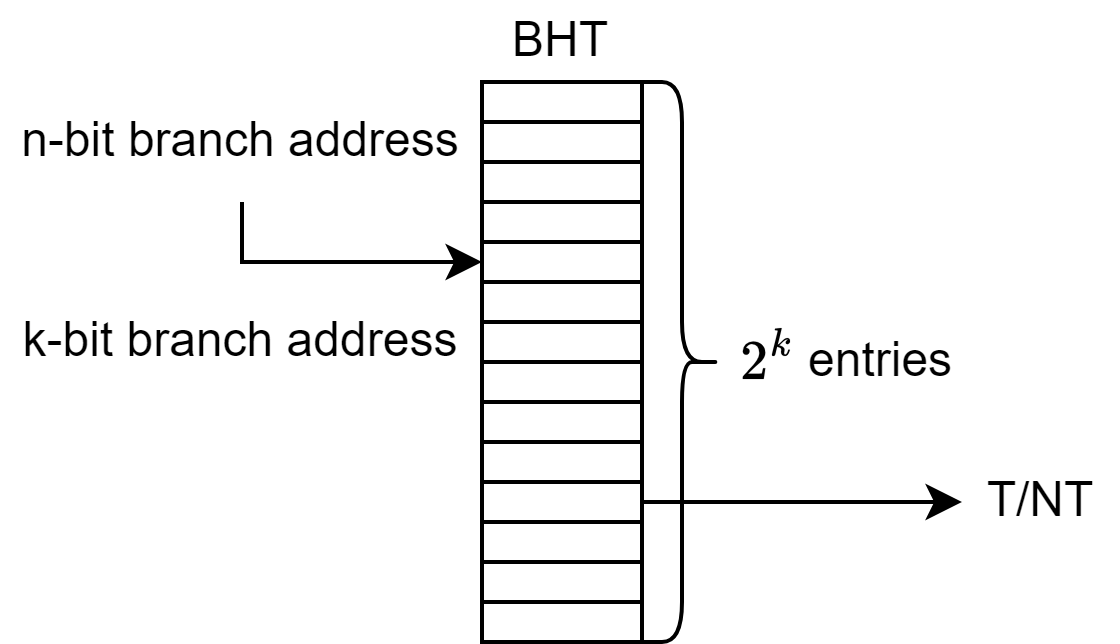
\includegraphics[width=0.5\linewidth]{images/bht.png}
    \caption{Branch history table structure}
\end{figure}
\paragraph*{Accuracy}
A misprediction arises when either the prediction is erroneous for a particular branch or when the same index has been referenced by two distinct branches, and the previous history pertains to the other branch.
To mitigate this issue, increasing the number of rows in the BHT or employing a hashing function (e.g., as in GShare) can be effective solutions.

\paragraph*{One-bit branch history table}
The 1-bit BHT exhibits a notable limitation in scenarios such as loop branches. 
Even if a branch is predominantly taken throughout a loop but is not taken once, the 1-bit BHT may mispredict twice instead of once.
This scheme results in two erroneous predictions:
\begin{itemize}
    \item At the conclusion of the loop iteration, where the prediction bit indicates a taken branch, contradicting the need to exit the loop.
    \item Upon re-entering the loop, following the first loop iteration's end, the branch should be taken to maintain loop execution. 
        However, the prediction bit suggests exiting the loop, stemming from the previous execution of the loop's final iteration where the prediction bit was flipped.
\end{itemize}

\paragraph*{Two-bit branch history table}
In the two-bit branch history table the prediction must fail twice before it undergoes alteration.
Within a loop branch, on the final iteration, there's no requirement to modify the prediction.
Each index in the table employs 2 bits to encode the four states of a finite state machine.

\paragraph*{N-bit branch history table}
For the $n$-bit Branch History Table, we require an n-bit saturating counter for each entry in the prediction buffer.
This counter has a range of values between $0$ and $2^n - 1$.
When the counter equals or exceeds half of its maximum value ($2^n - 1$), the branch is predicted as taken; otherwise, it's predicted as untaken.
Similar to the 2-bit scheme, the counter increments with a taken branch and decrements with an untaken branch.
Research on $n$-bit predictors indicates that 2-bit predictors perform nearly as effectively.

\subsection{Branch target predictor}
\paragraph*{Branch target buffer}
Branch target buffer (BTB), also known as branch target predictor, functions as a cache that stores the anticipated branch target address for the instruction following a branch.
During the Instruction Fetch (IF) stage, the BTB is accessed using the instruction address of the fetched instruction, which could potentially be a branch, to index the cache.
Typical entries in the BTB include:
\begin{itemize}
    \item The exact address of a branch.
    \item The predicted target address.
\end{itemize}
The predicted target address is typically represented as PC-relative.
\begin{figure}[H]
    \centering
    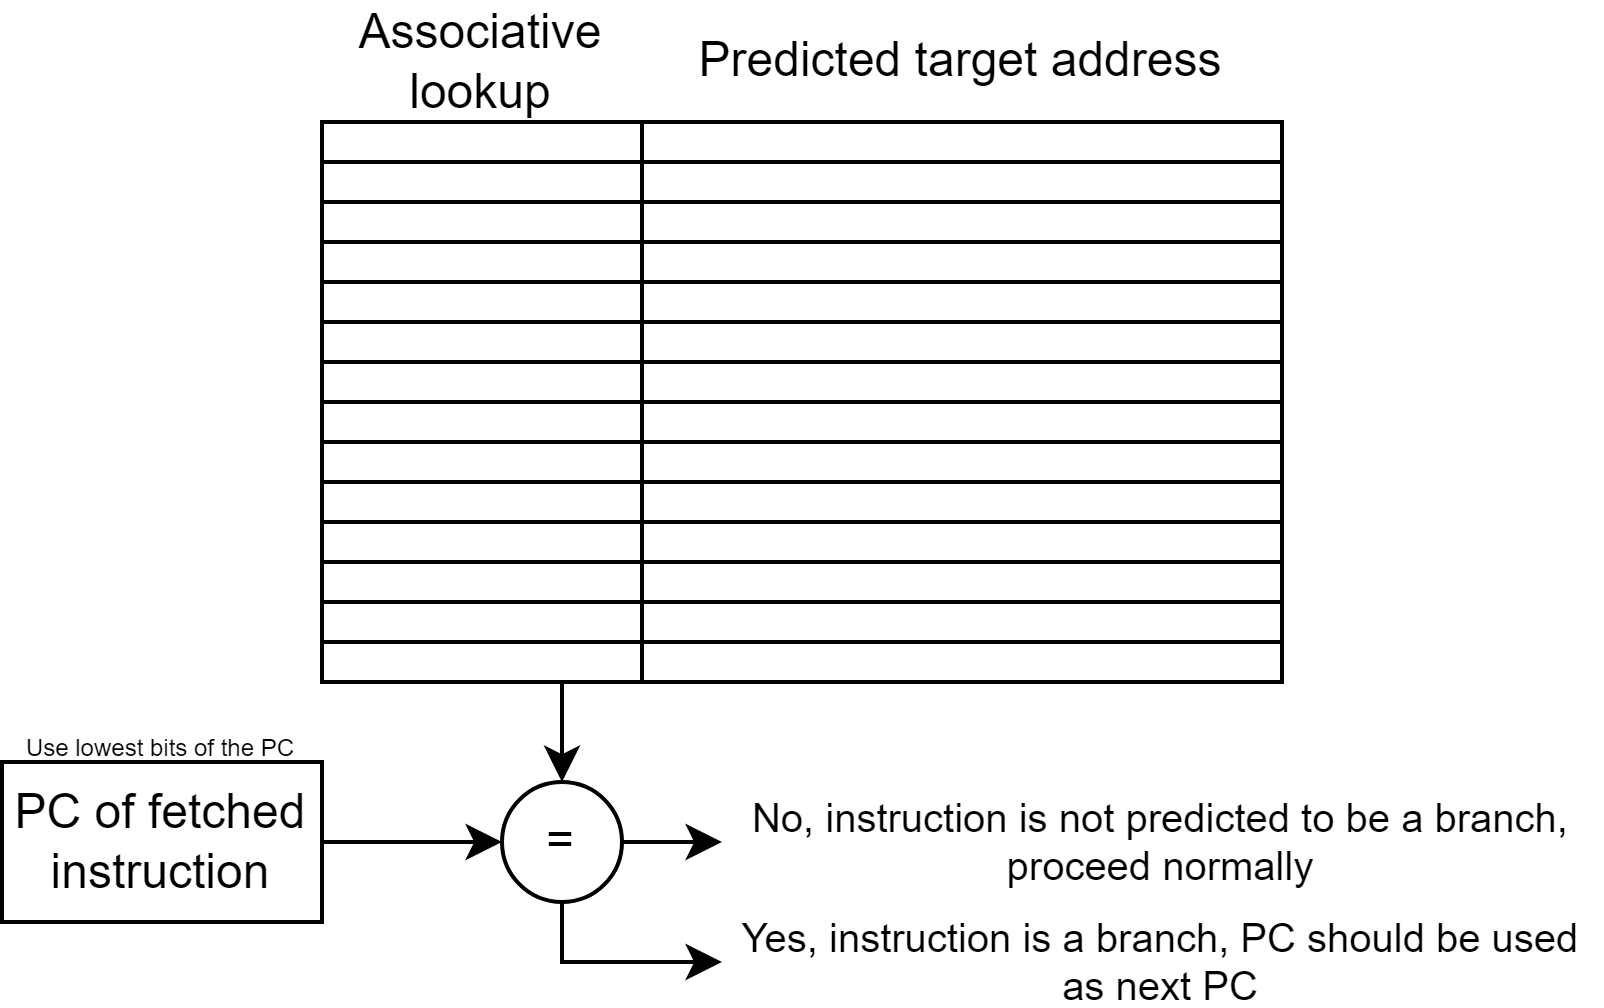
\includegraphics[width=0.5\linewidth]{images/btb.png}
    \caption{Branch target buffer structure}
\end{figure}

\subsection{Correlating branch predictors}
BHT predictors rely solely on the recent behavior of a single branch to forecast its future behavior.

Correlating branch predictors, on the other hand, operate on the principle that recent branches exhibit correlations. 
This means that the recent behavior of not just the current branch under consideration but also other branches can influence the prediction of the current branch.

Predictors that leverage the behavior of other branches to make predictions are known as correlating predictors or 2-level predictors.

In a general ($m, n$) correlating predictor, the system stores the last m branches to select from $2^m$ branch history tables (BHTs), with each BHT being an $n$-bit predictor.

\paragraph*{Accuracy}
A 2-bit predictor lacking global history can be regarded as a ($0, 2$) predictor.
Comparing the performance of a 2-bit simple predictor featuring four thousand entries with that of a ($2,2$) correlating predictor with one thousand entries.
The (2,2) predictor not only surpasses the simple 2-bit predictor having the same total number of bits (four thousand total bits), but it frequently outperforms a 2-bit predictor regardless of the number of entries.

\paragraph*{Two-level adaptive branch predictors}
The first level history is stored in one or more $k$-bit shift registers known as the branch history register (BHR), which records the outcomes of the $k$ most recent branches.
The second level history is stored in one or more tables called pattern history table (PHT), consisting of two-bit saturating counters.
The BHR is utilized to index the PHT to determine which 2-bit counter to use.

Once the two-bit counter is selected, the prediction is made using the same method as in the two-bit counter scheme.
We may have: 
\begin{itemize}
    \item \textit{BHT}: local predictor, indexed by the low-order bits of the program counter (branch address).
    \item \textit{GAs}: local and global predictor, a 2-level predictor: PHT indexed by the content of BHR (global history).
    \item \textit{GShare}: local XOR global information, indexed by the exclusive OR of the low-order bits of the program counter (branch address) and the content of BHR (global history).
\end{itemize}